\documentclass[11pt]{amsart}
\usepackage{geometry}                % See geometry.pdf to learn the layout options. There are lots.
\geometry{letterpaper}                   % ... or a4paper or a5paper or ... 
%\geometry{landscape}                % Activate for for rotated page geometry
%\usepackage[parfill]{parskip}    % Activate to begin paragraphs with an empty line rather than an indent
\usepackage{graphicx}
\usepackage{amssymb,amsmath}
\usepackage{tabularx}
\usepackage{array}
%\DeclareGraphicsRule{.tif}{png}{.png}{`convert #1 `dirname #1`/`basename #1 .tif`.png}

\title{Brief Article}
\author{The Author}
%\date{}                                           % Activate to display a given date or no date

\begin{document}
\maketitle
%\section{}
%\subsection{}
\begin{tabular}{|m{1in}|m{1in}|}
  image & matrix \\
  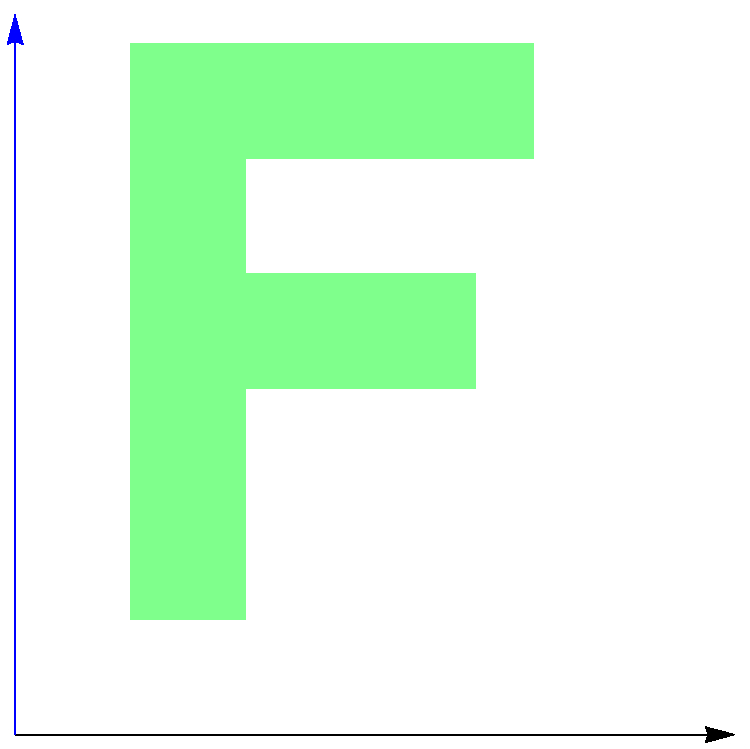
\includegraphics[ width = 1.5in ]{pdf/coordinate_systems/Ia}   & $\itwo$ \\
  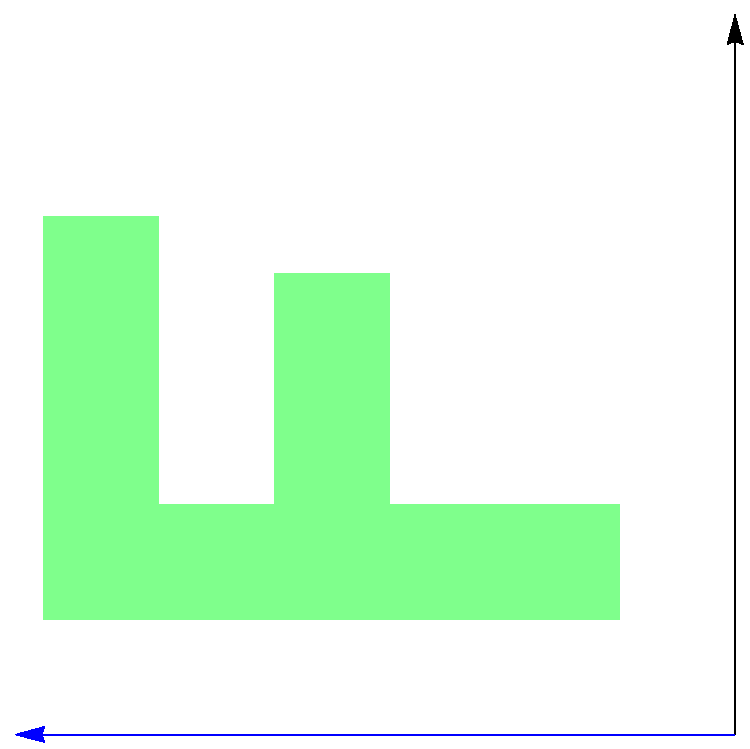
\includegraphics[ width = 1.5in ]{pdf/coordinate_systems/IIa}  & $\itwo$ \\
\end{tabular}


\begin{tabularx}{\textwidth}{YXZW}
\toprule
Cell with text aligned to the left & 1 & 2 & 3\\\midrule
4 & Cell with justified text & 5 & 6\\\midrule
7 & 8 & Cell with centered text & 9\\\midrule
10 & 11 & 12 & Cell with text aligned to the right\\\bottomrule
\end{tabularx}

\renewcommand{\tabularxcolumn}[1]{>{\arraybackslash}m{#1}}
\begin{tabularx}{\textwidth}{YXZW}
\toprule Cell with text aligned to the left & 1 & 2 & 3\\\midrule 4 &
Cell with justified text & 5 & 6\\\midrule 7 & 8 & Cell with centeredtext & 9\\\midrule 10 & 11 & 12 & Cell with text aligned to the
right \\\ bottomrule
\end{tabularx}

\end{document}  